In the following section we will showcase the resulting workflow of our prototype and the evaluation results for our repository containing the QuixBugs benchmark problems.
\section{Showcase of workflow}
%TODO reference to requirements
To integrate the APR system into a repository living on GitHub we need to move the pipeline with its filter script to the dedicated github action workflow directory.
---IMAGE OF WORKFLOW IN PLACE
% \begin{figure}[H]
%     \centering
%     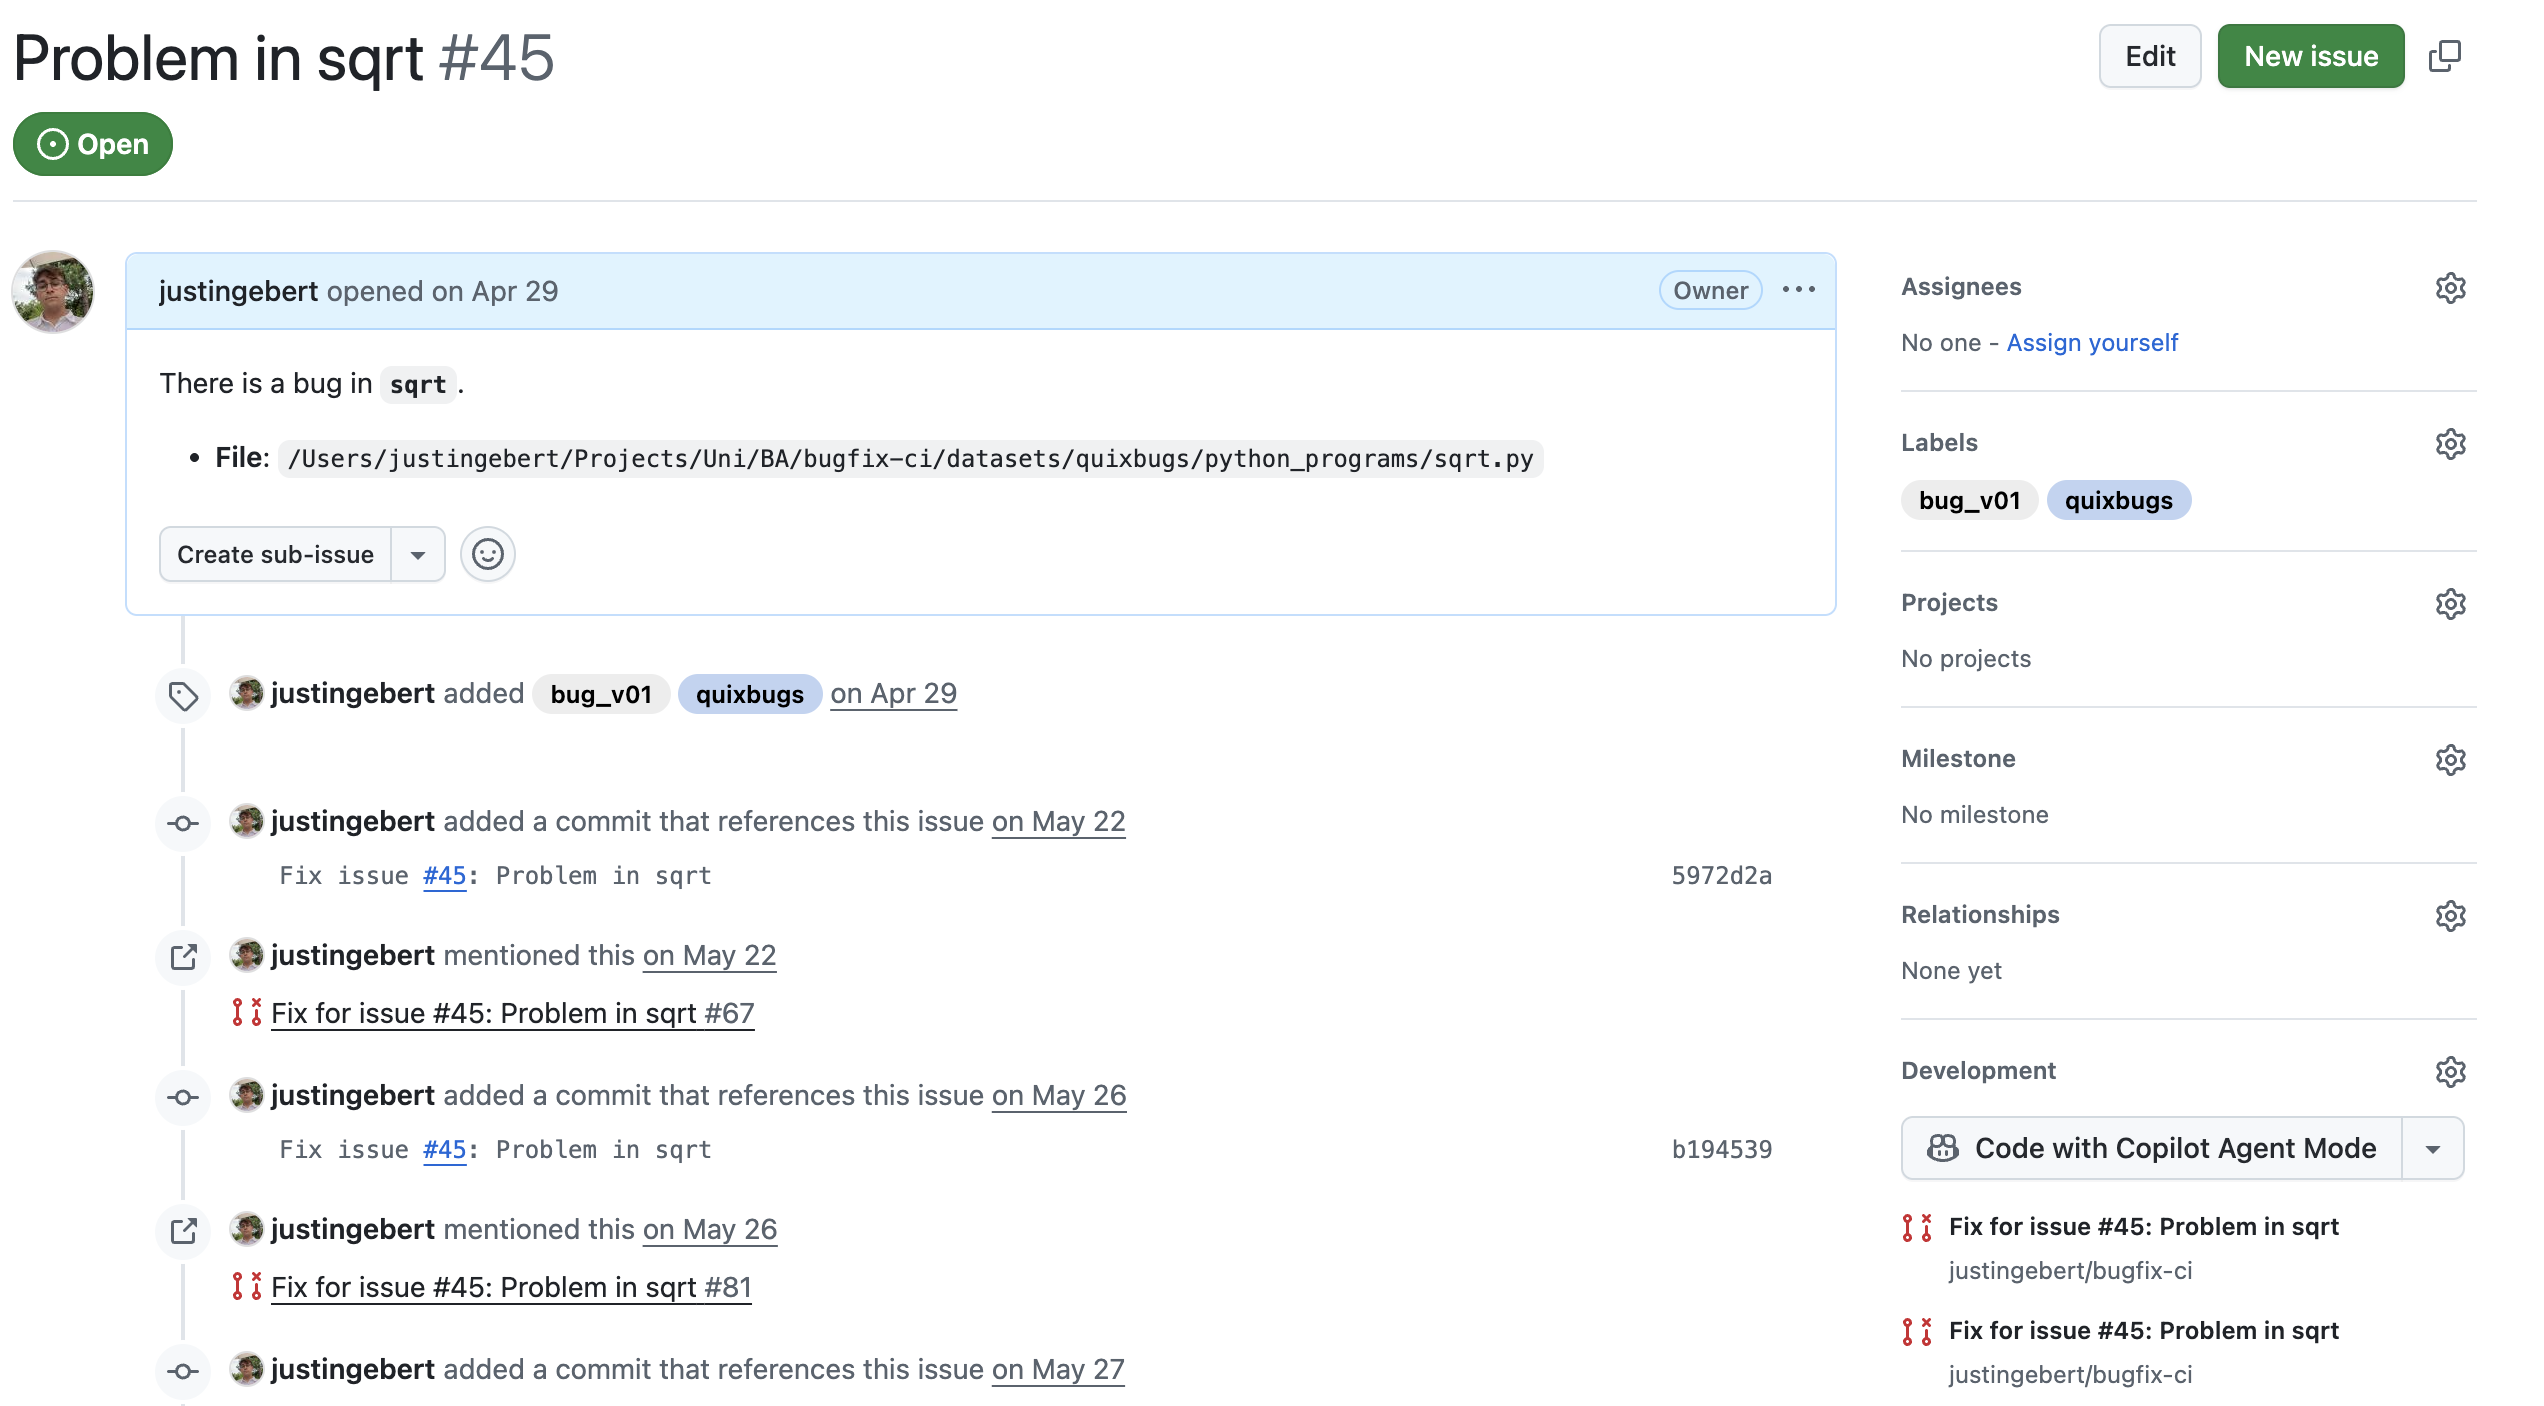
\includegraphics[width=1\textwidth]{images/github/GitHub Issue.png}
%     \caption{Example of a GitHub Issue}
%     \label{fig:gh-issue}
% \end{figure}

The follwing repository secrets need to be set in the repository settings GITHUB\_TOKEN: a personal access token with write access to the repository LLM\_API\_KEY: the API key for the LLM provider e.g. OpenAI, Gemini, etc.

When the workflow is in place the APR system is ready to go. Optionally its default behavior can be altered by adding a configuration file (called: bugfix.yml) to the root of the repository.
---EXAMPLE OF CONFIG
% \begin{figure}[H]
%     \centering
%     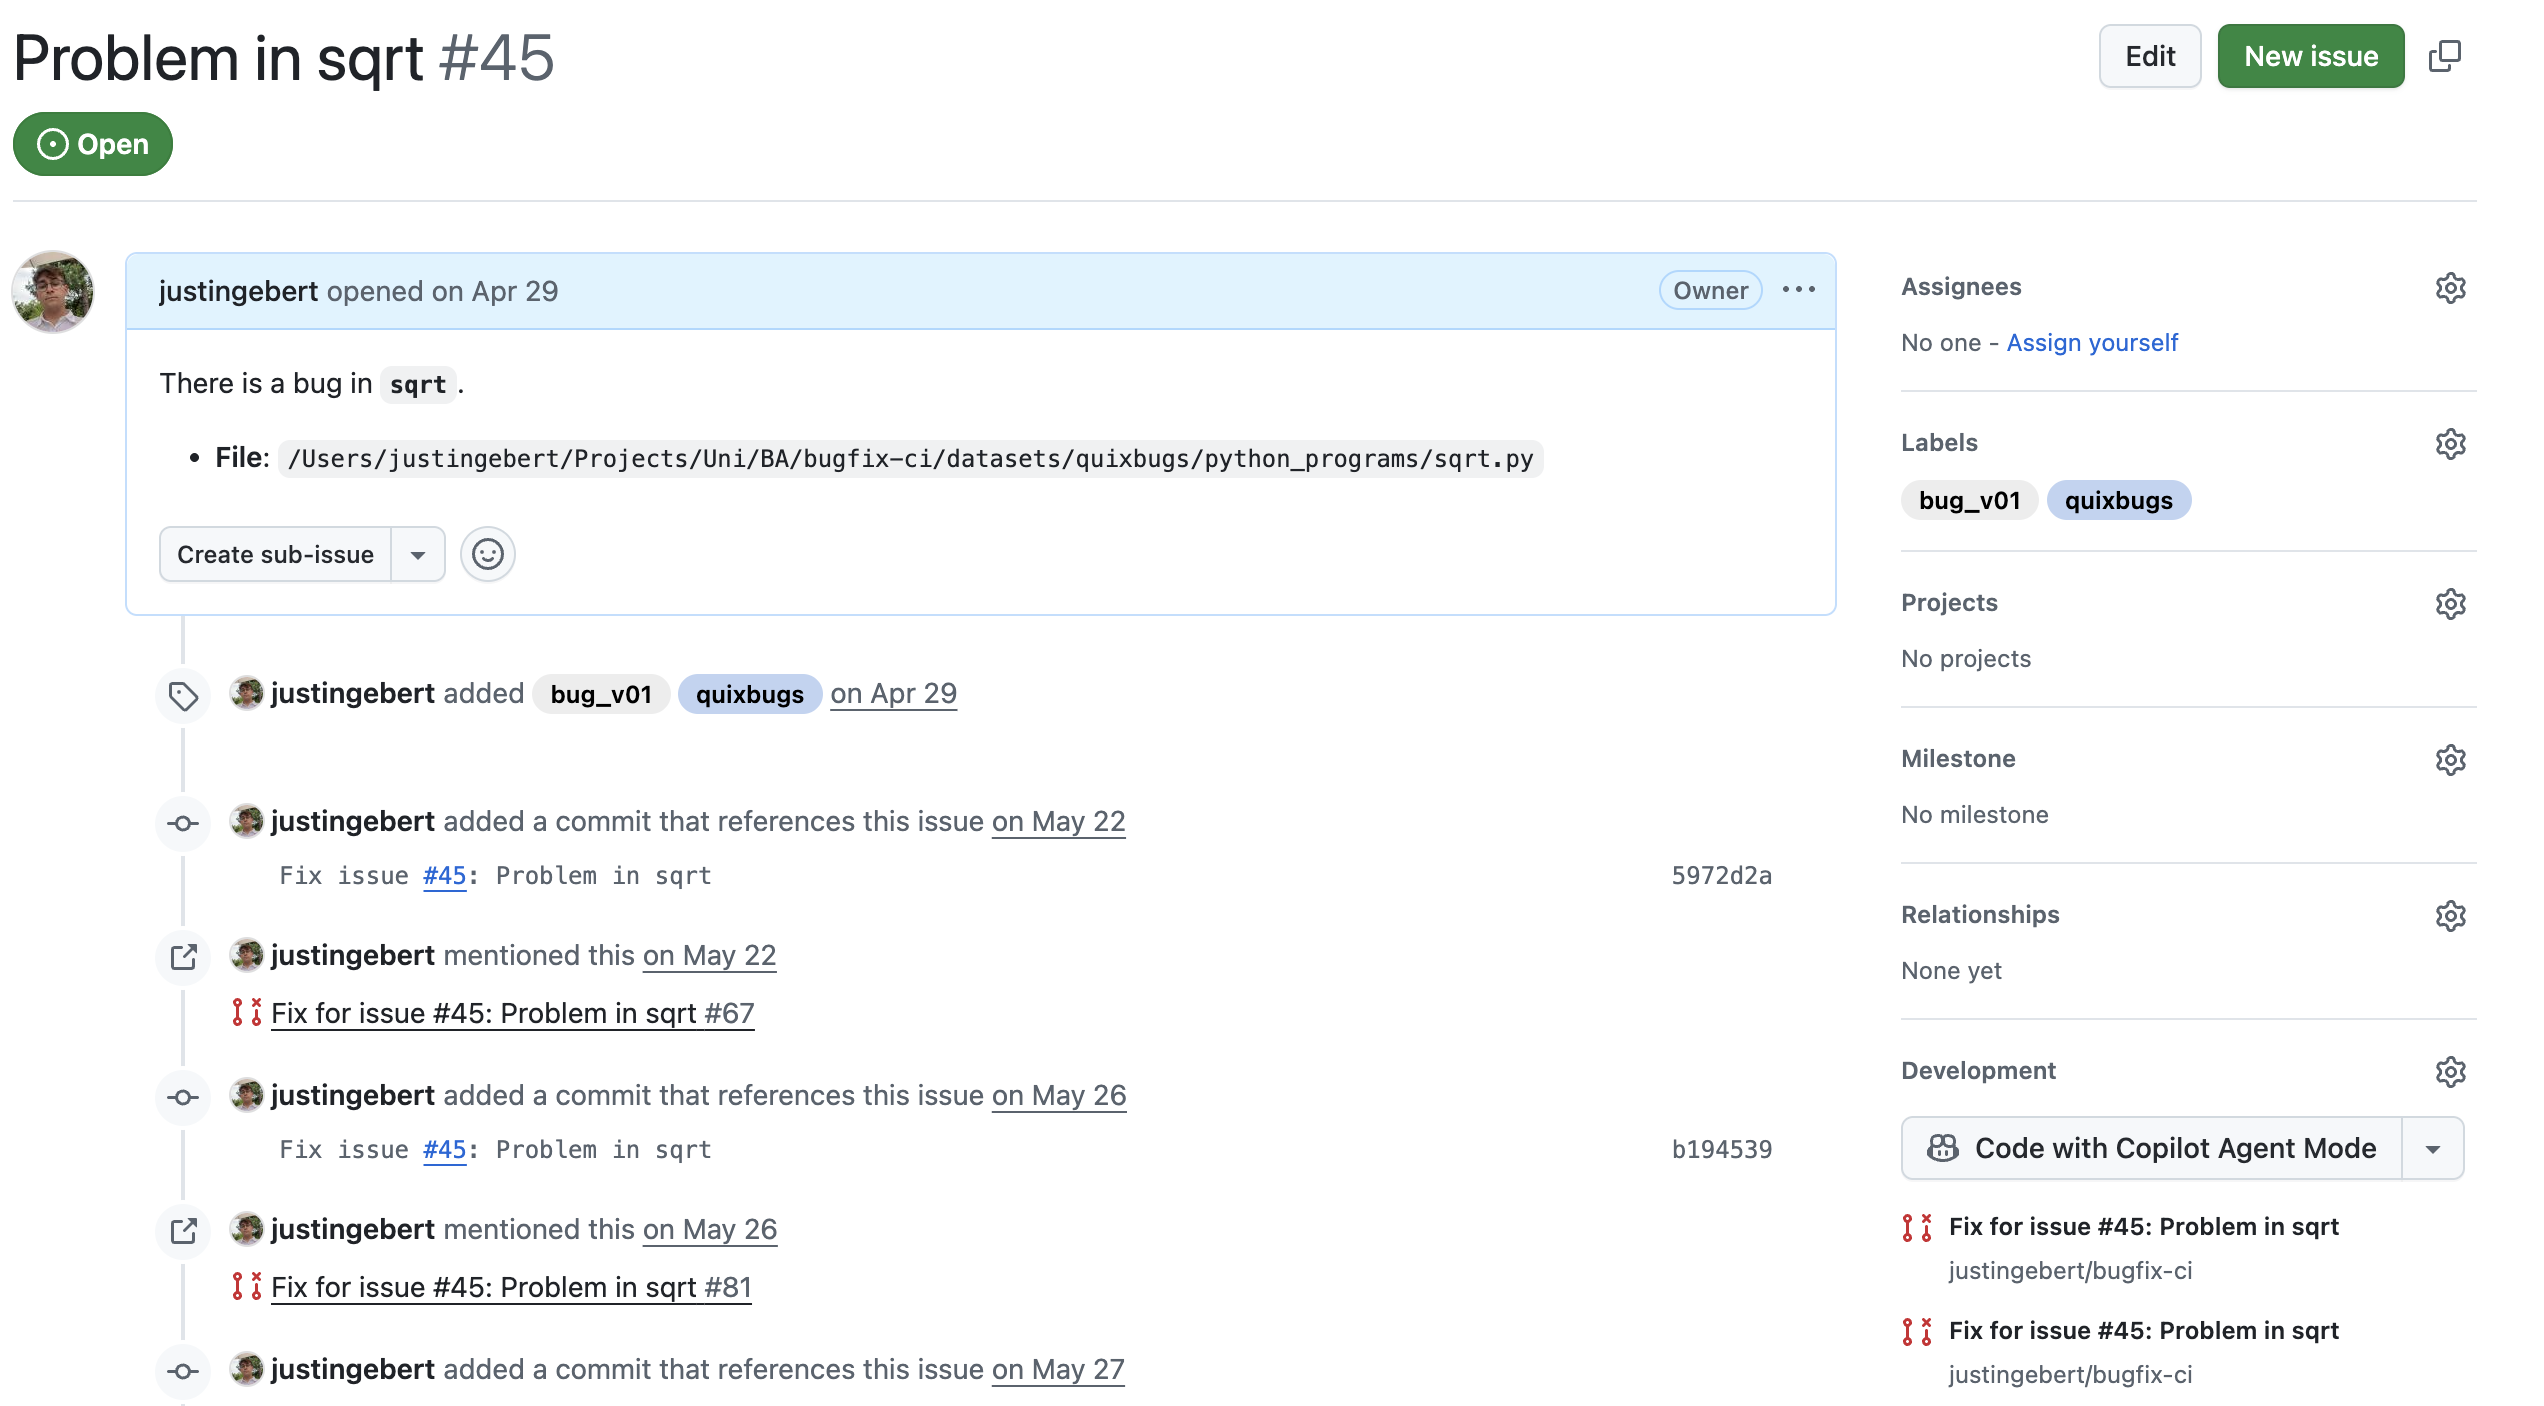
\includegraphics[width=1\textwidth]{images/github/GitHub Issue.png}
%     \caption{Example of a GitHub Issue}
%     \label{fig:gh-issue}
% \end{figure}

Now when an issue is created and labeled with the default label "bug" (or a custom label defined in the configuration file) the APR system will be triggered and start the bug fixing process. Manual triggering is also possible by using the "Run workflow" button in the GitHub actions tab of the repository.
---IMAGE OF ISSUE BEING CREATED OR MANUALLY TRIGGERED
% \begin{figure}[H]
%     \centering
%     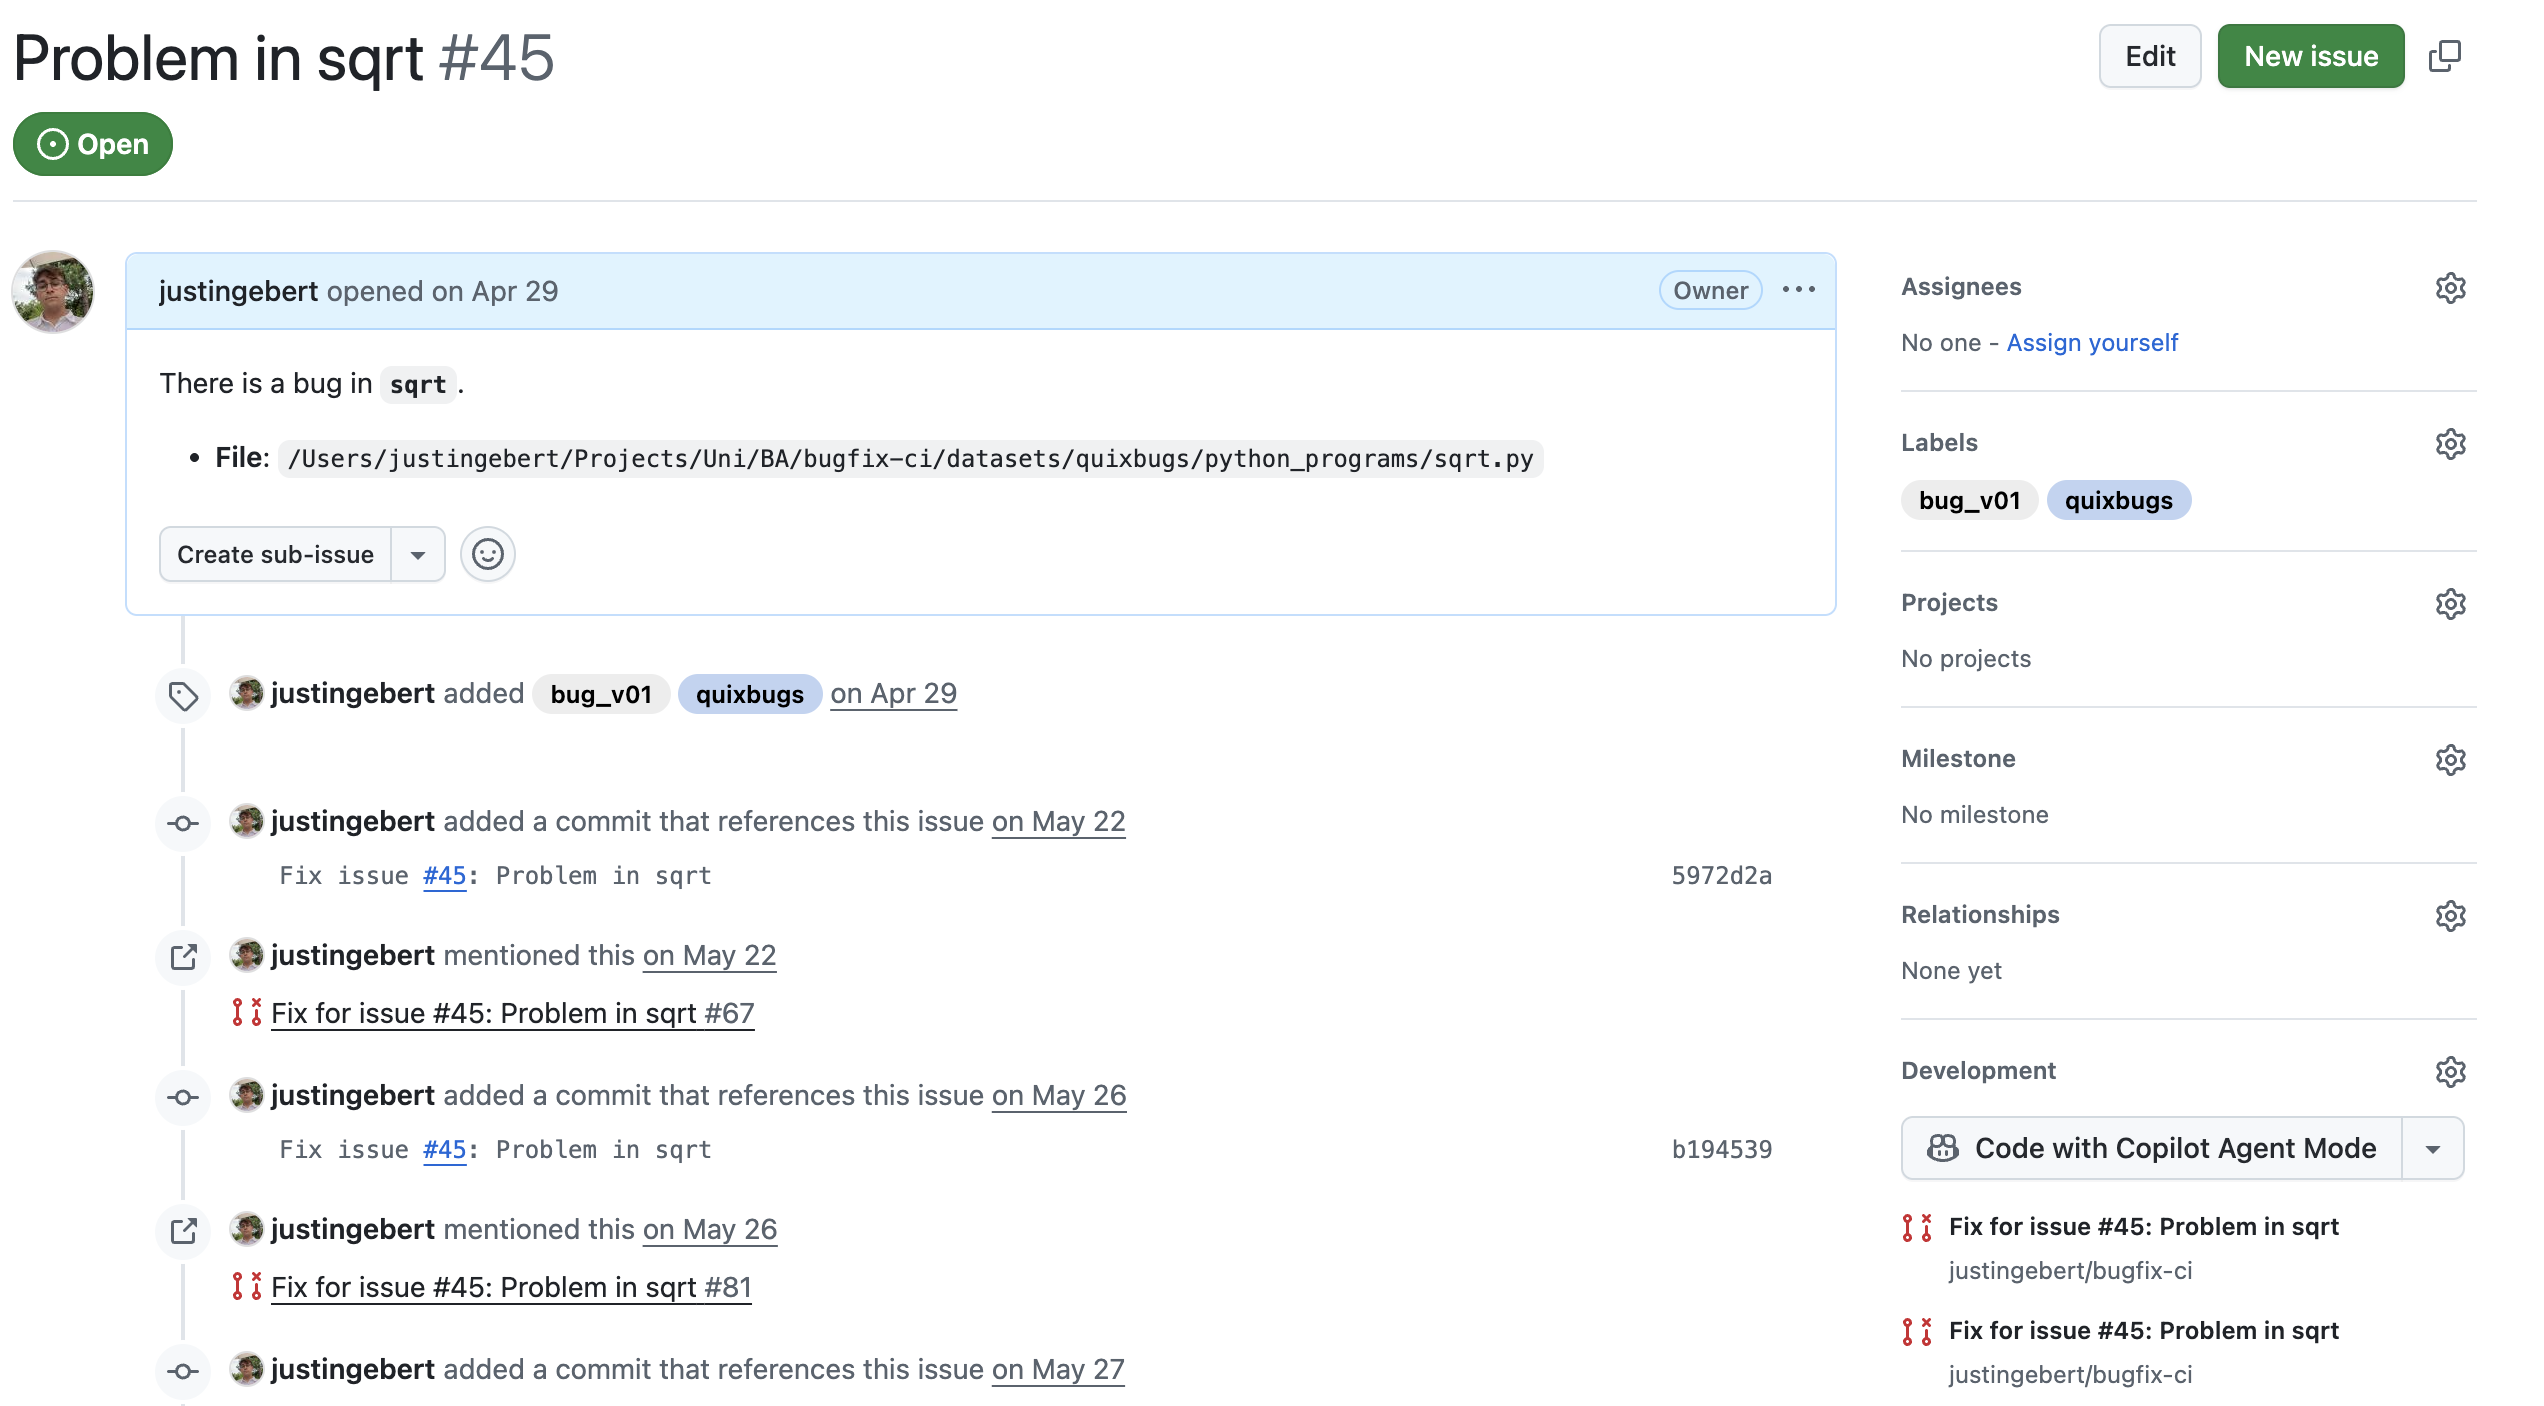
\includegraphics[width=1\textwidth]{images/github/GitHub Issue.png}
%     \caption{Example of a GitHub Issue}
%     \label{fig:gh-issue}
% \end{figure}

After the workflow is triggered and relevant issues are found the APR system start as a run of the GitHub action workflow.
---IMAGE OF RUN BEING STARTED
% \begin{figure}[H]
%     \centering
%     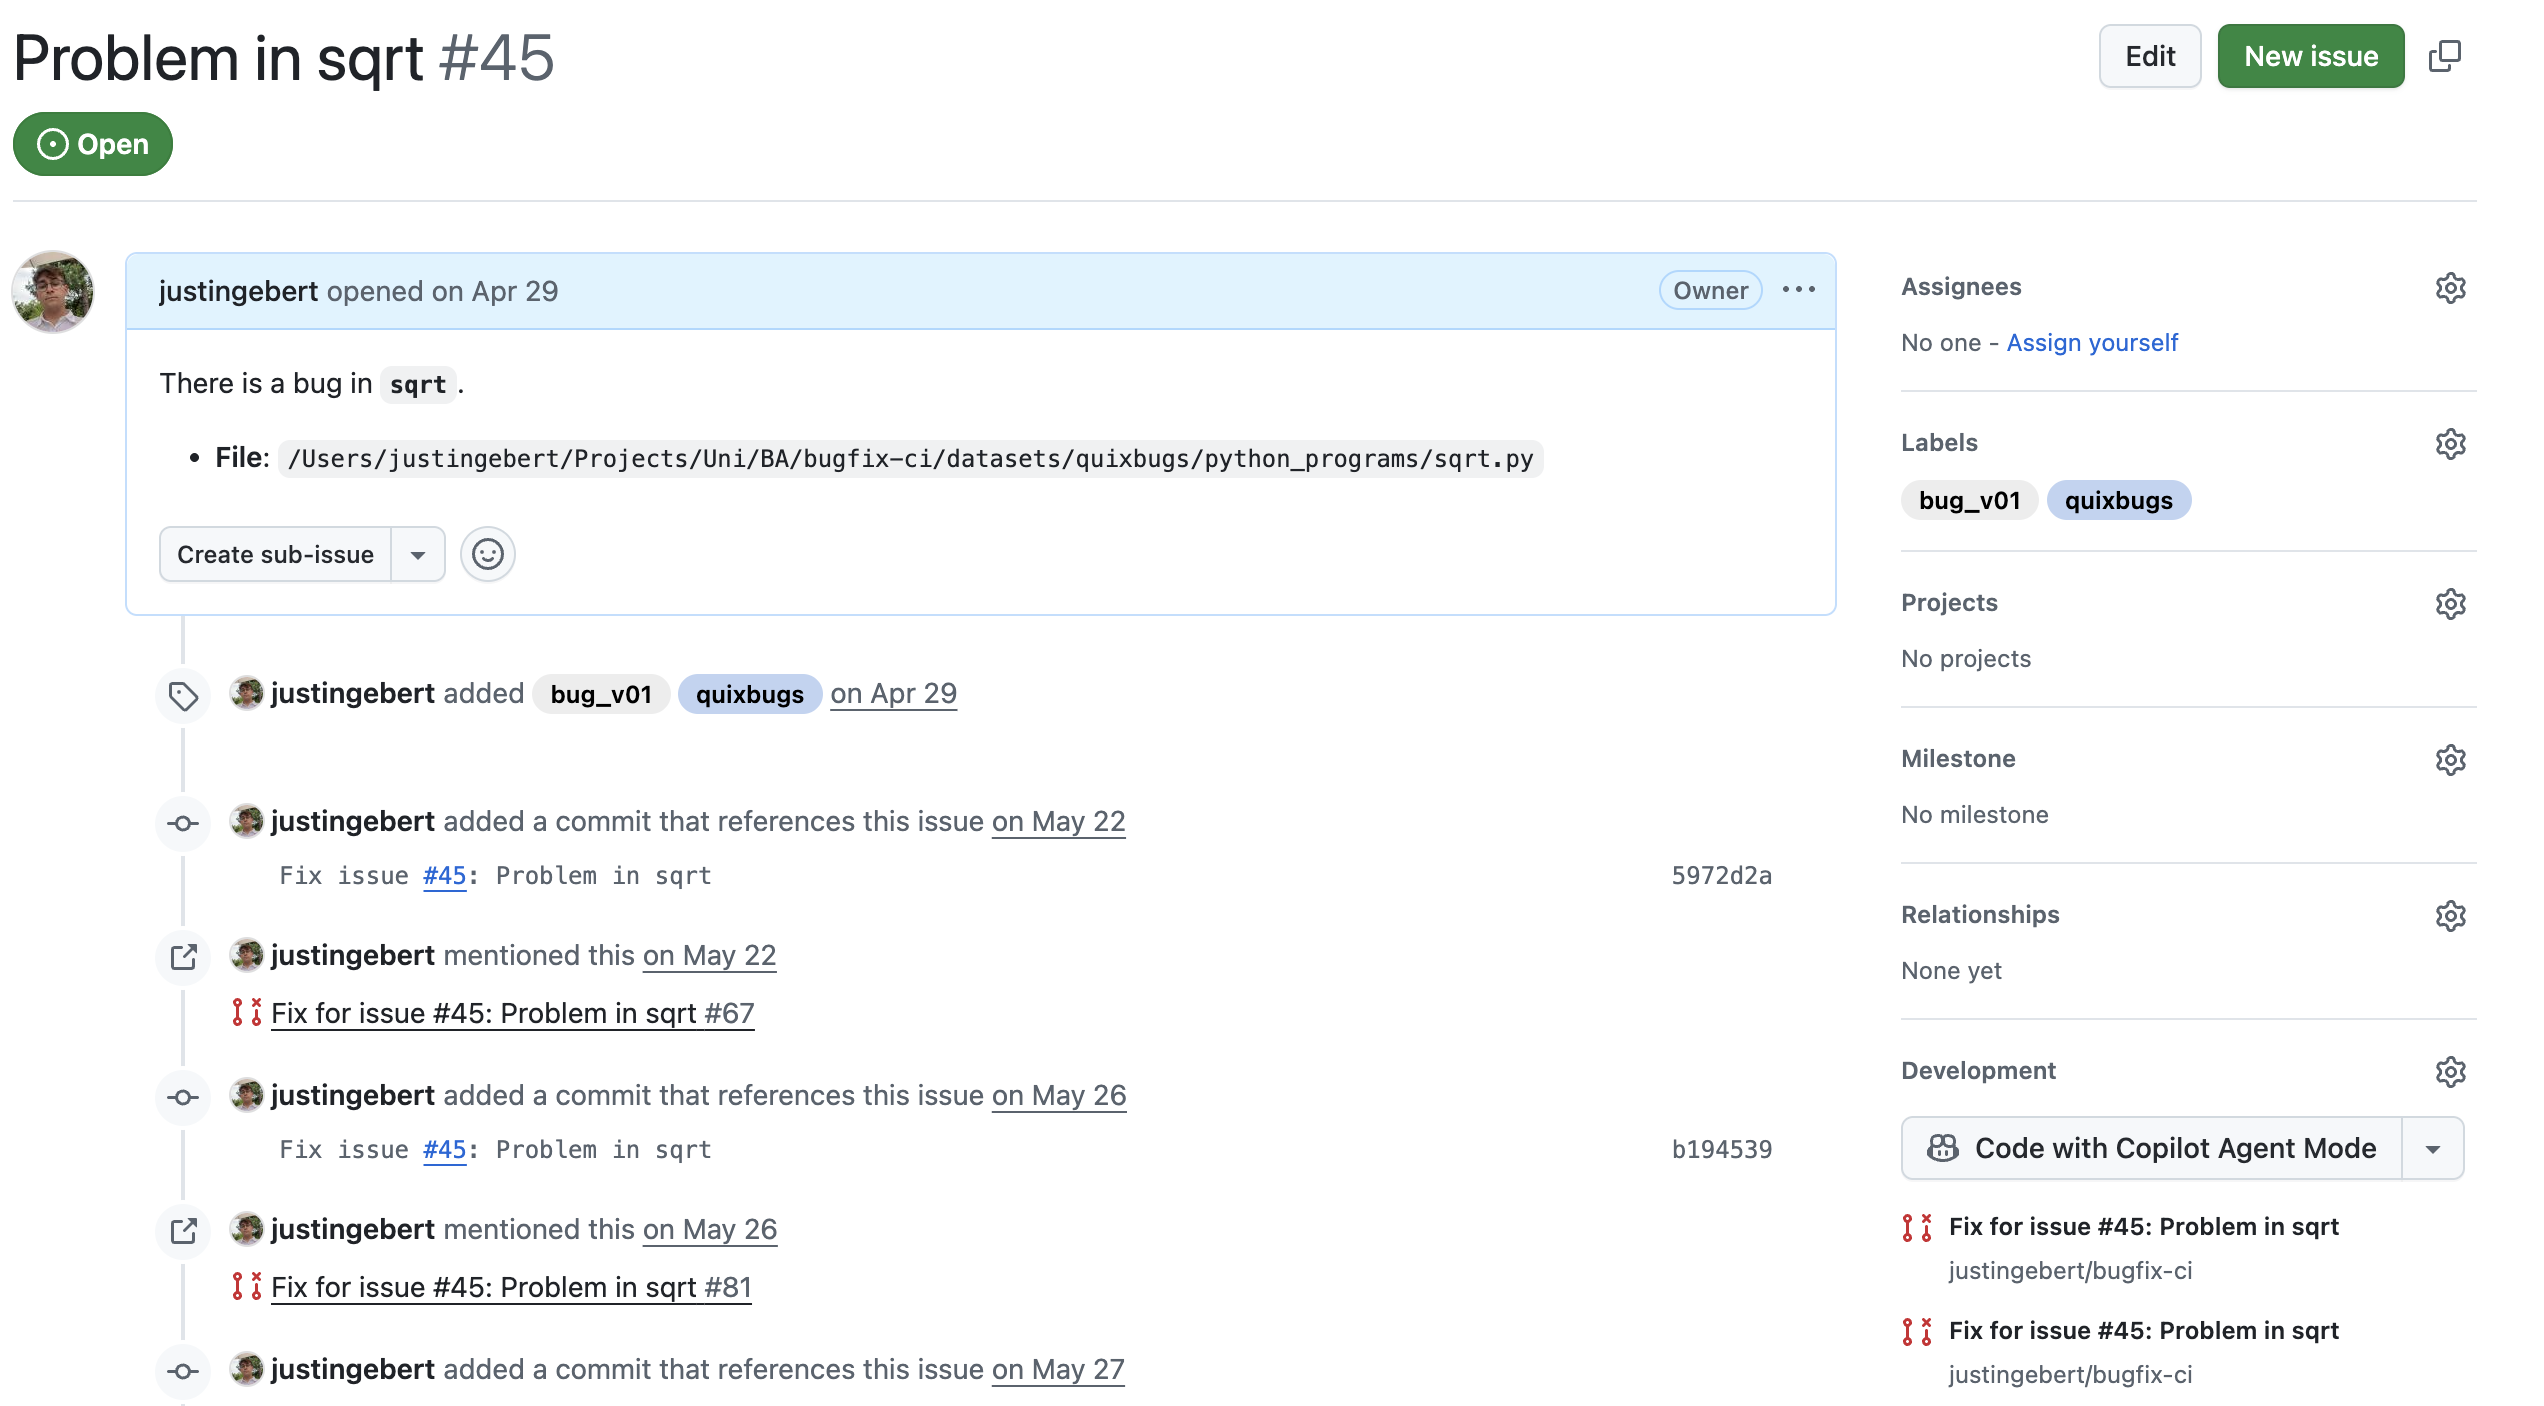
\includegraphics[width=1\textwidth]{images/github/GitHub Issue.png}
%     \caption{Example of a GitHub Issue}
%     \label{fig:gh-issue}
% \end{figure}

When the automatic bug fixing process has completed there are two possible outcomes:
Pull Request with patch for bug and link to the issue.
---IMAGE OF PULL REQUEST
% \begin{figure}[H]
%     \centering
%     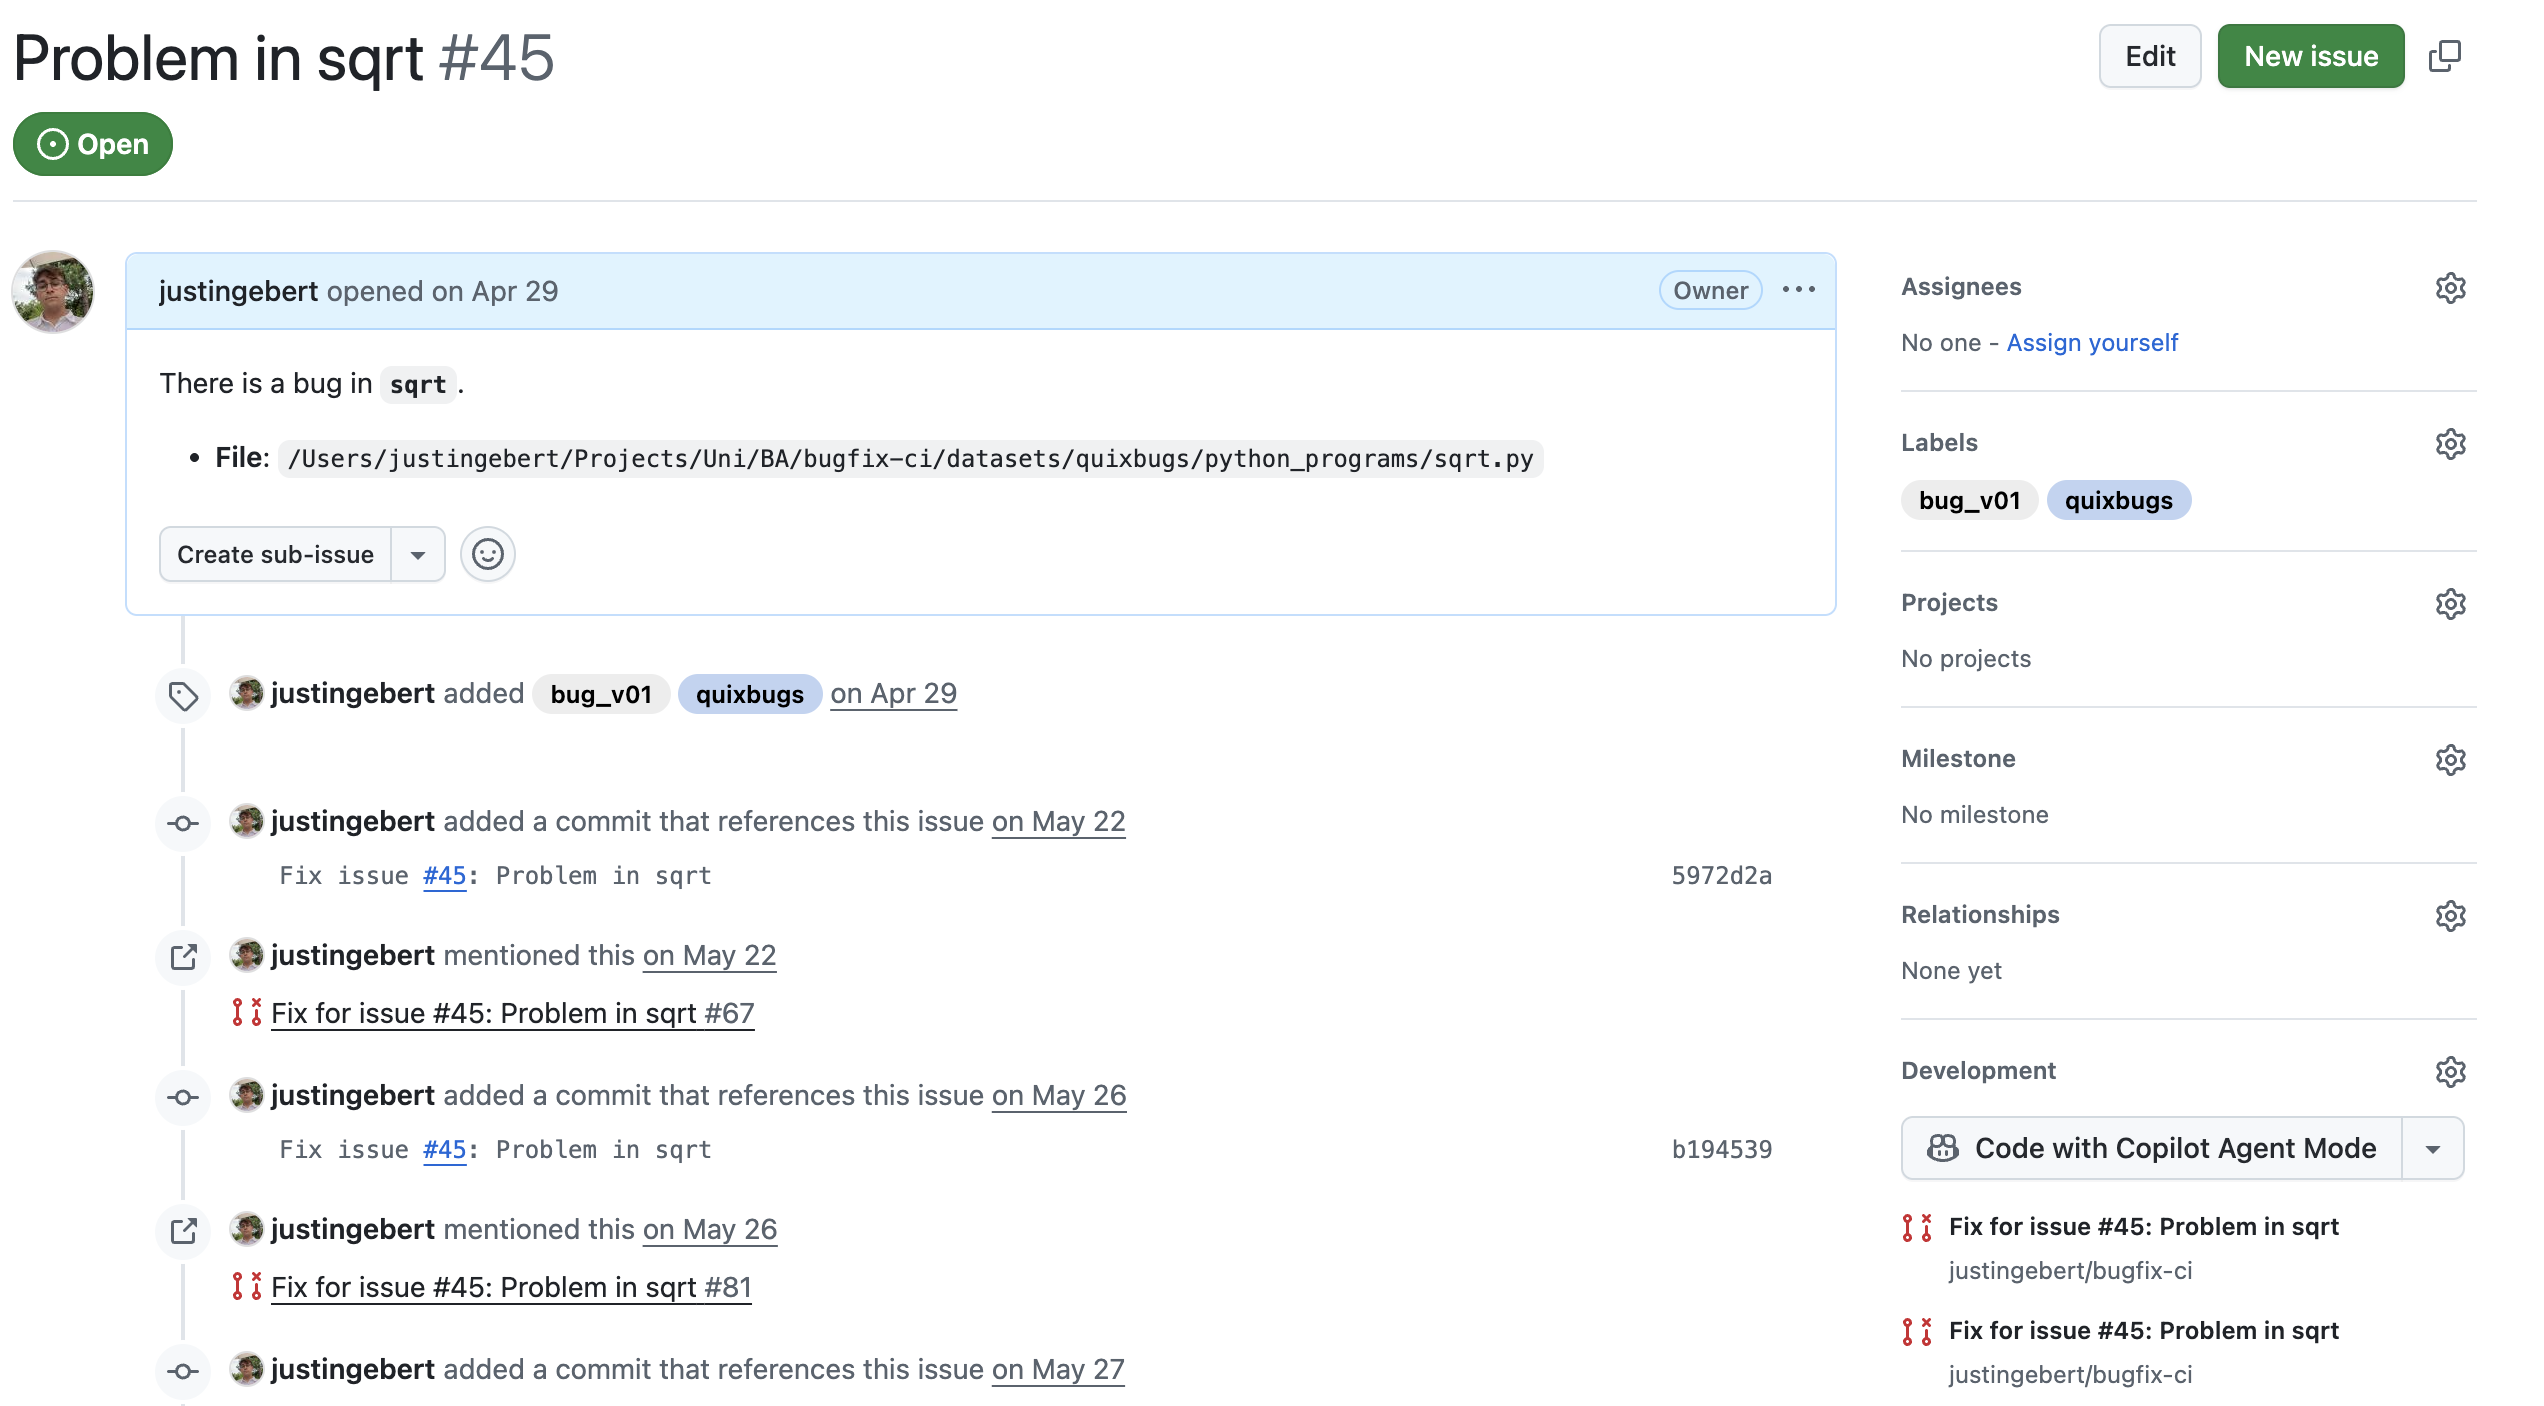
\includegraphics[width=1\textwidth]{images/github/GitHub Issue.png}
%     \caption{Example of a GitHub Issue}
%     \label{fig:gh-issue}
% \end{figure}

or a comment on the issue that bug fixing failed after all attempts.
---IMAGE OF COMMENT ON ISSUE
% \begin{figure}[H]
%     \centering
%     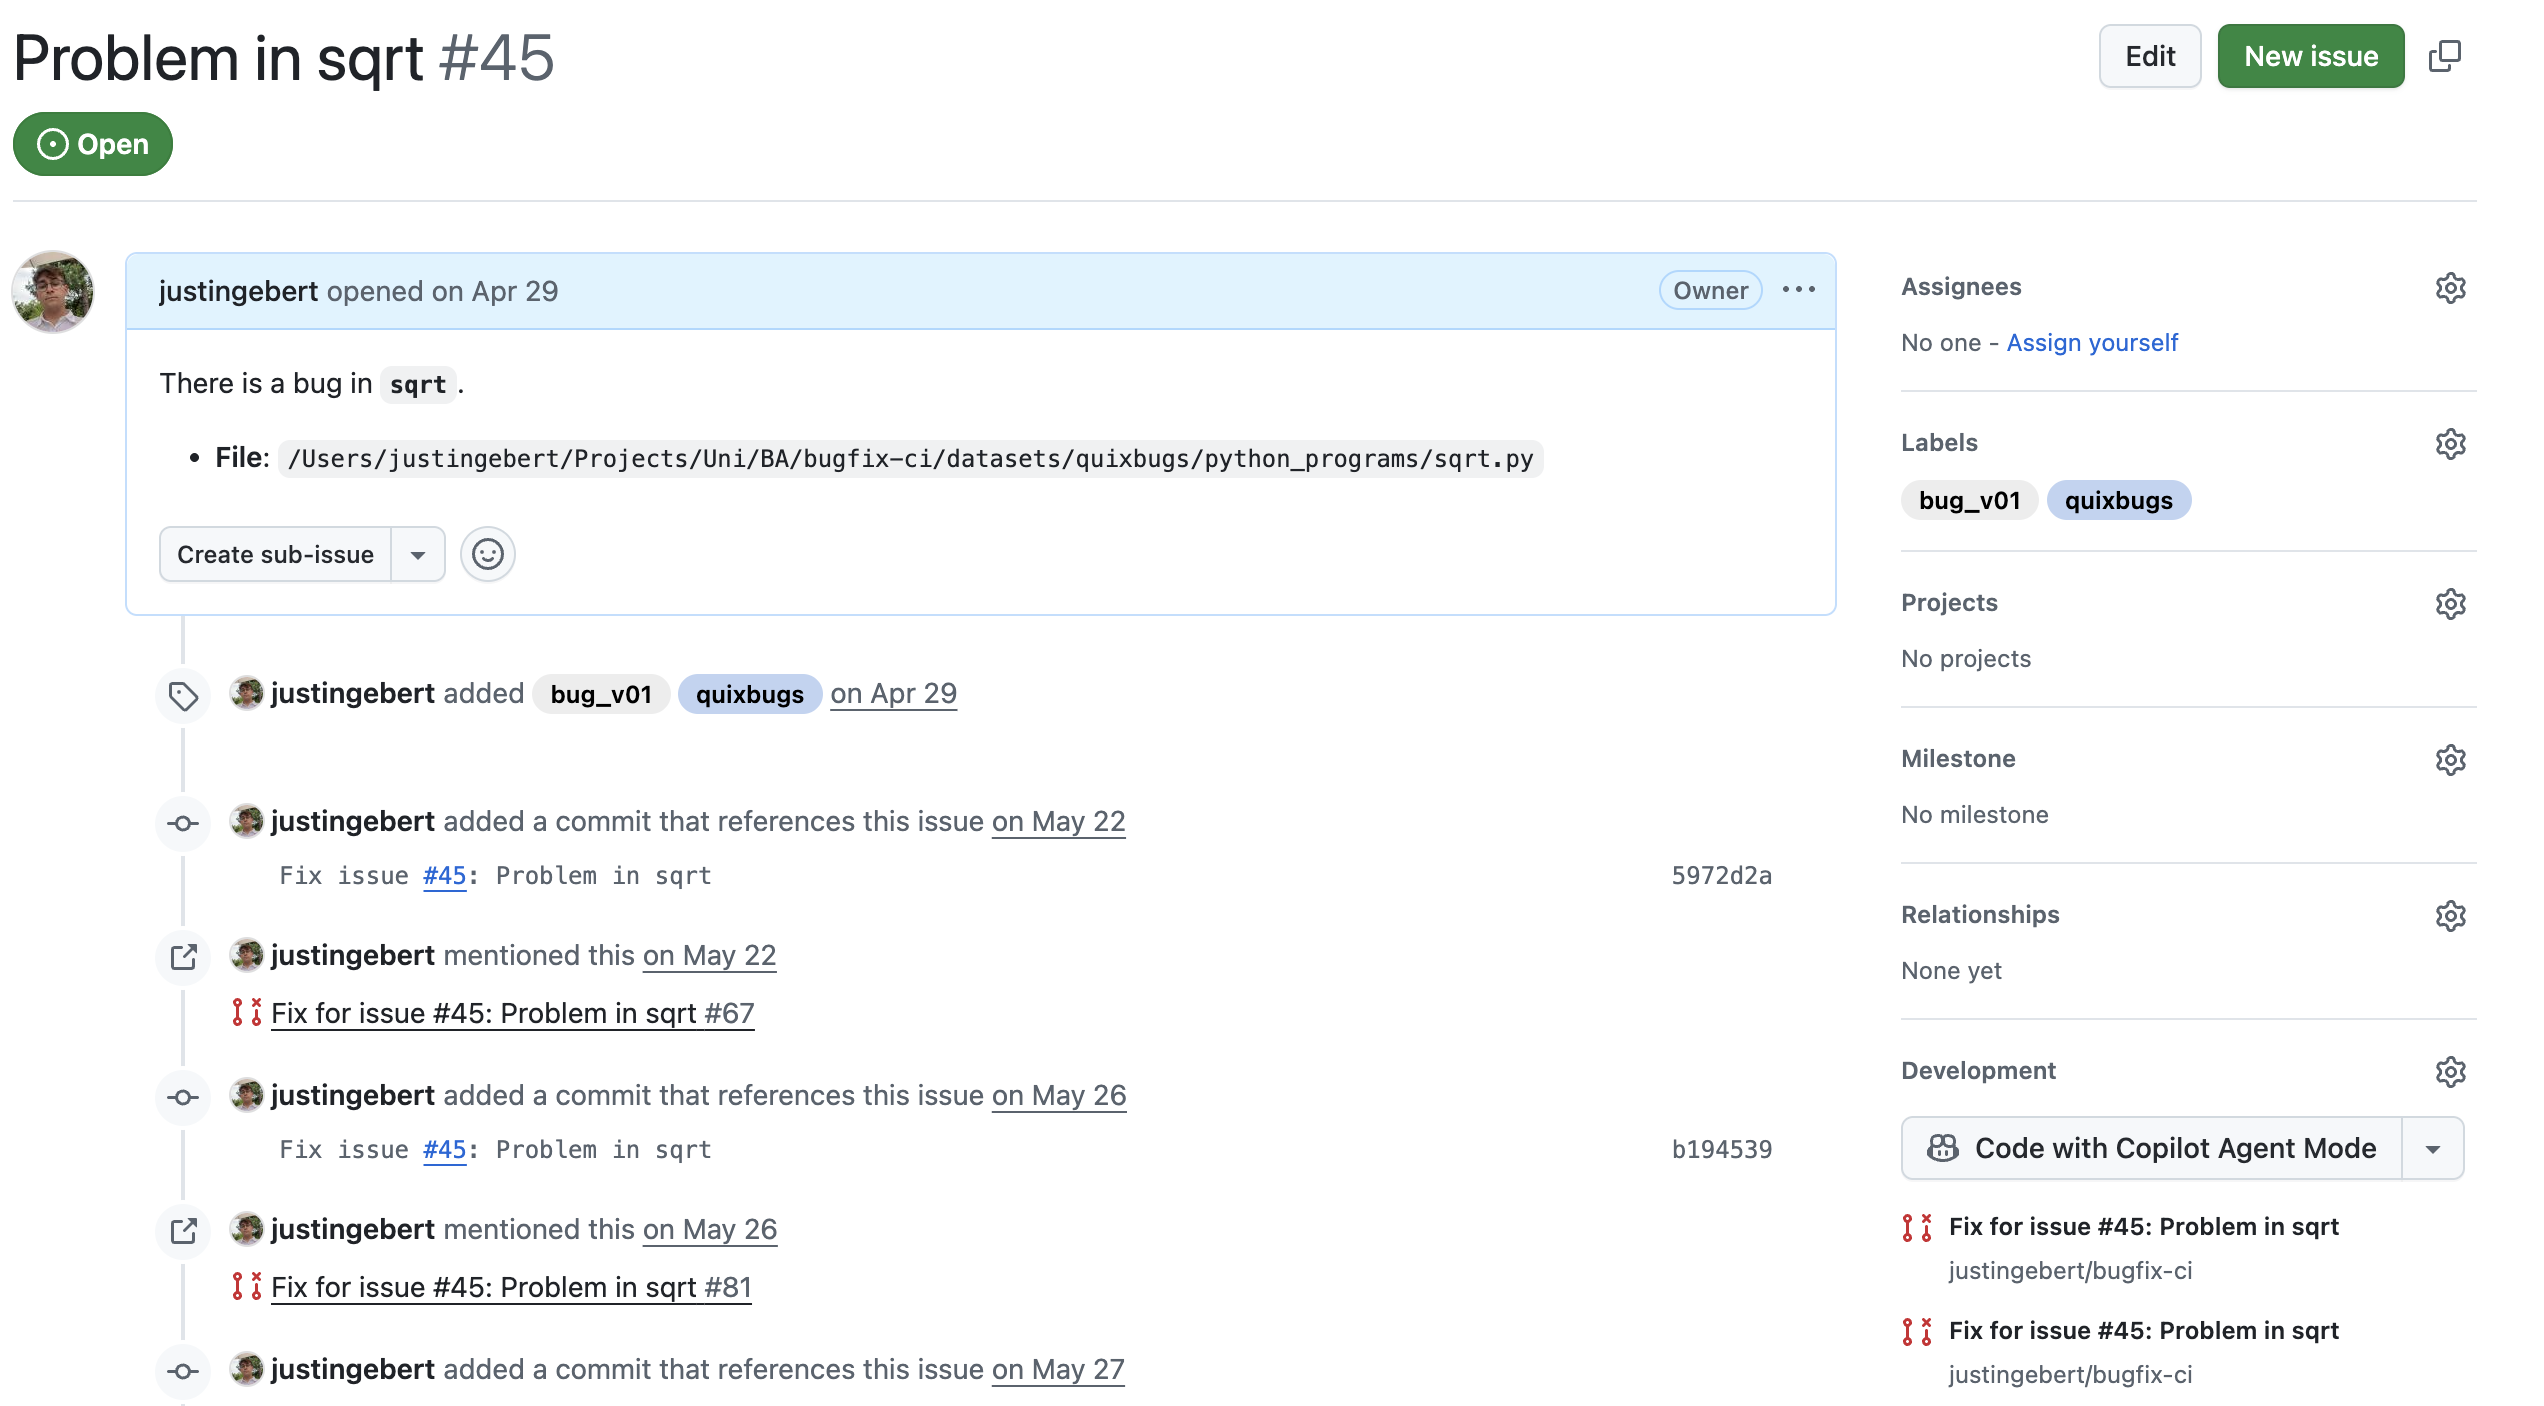
\includegraphics[width=1\textwidth]{images/github/GitHub Issue.png}
%     \caption{Example of a GitHub Issue}
%     \label{fig:gh-issue}
% \end{figure}

After the Workflow finishes metrics and logs are available for download in the action.
(during a run logs are live streamed in the Workflow run)
---IMAGE OF LOGS
% \begin{figure}[H]
%     \centering
%     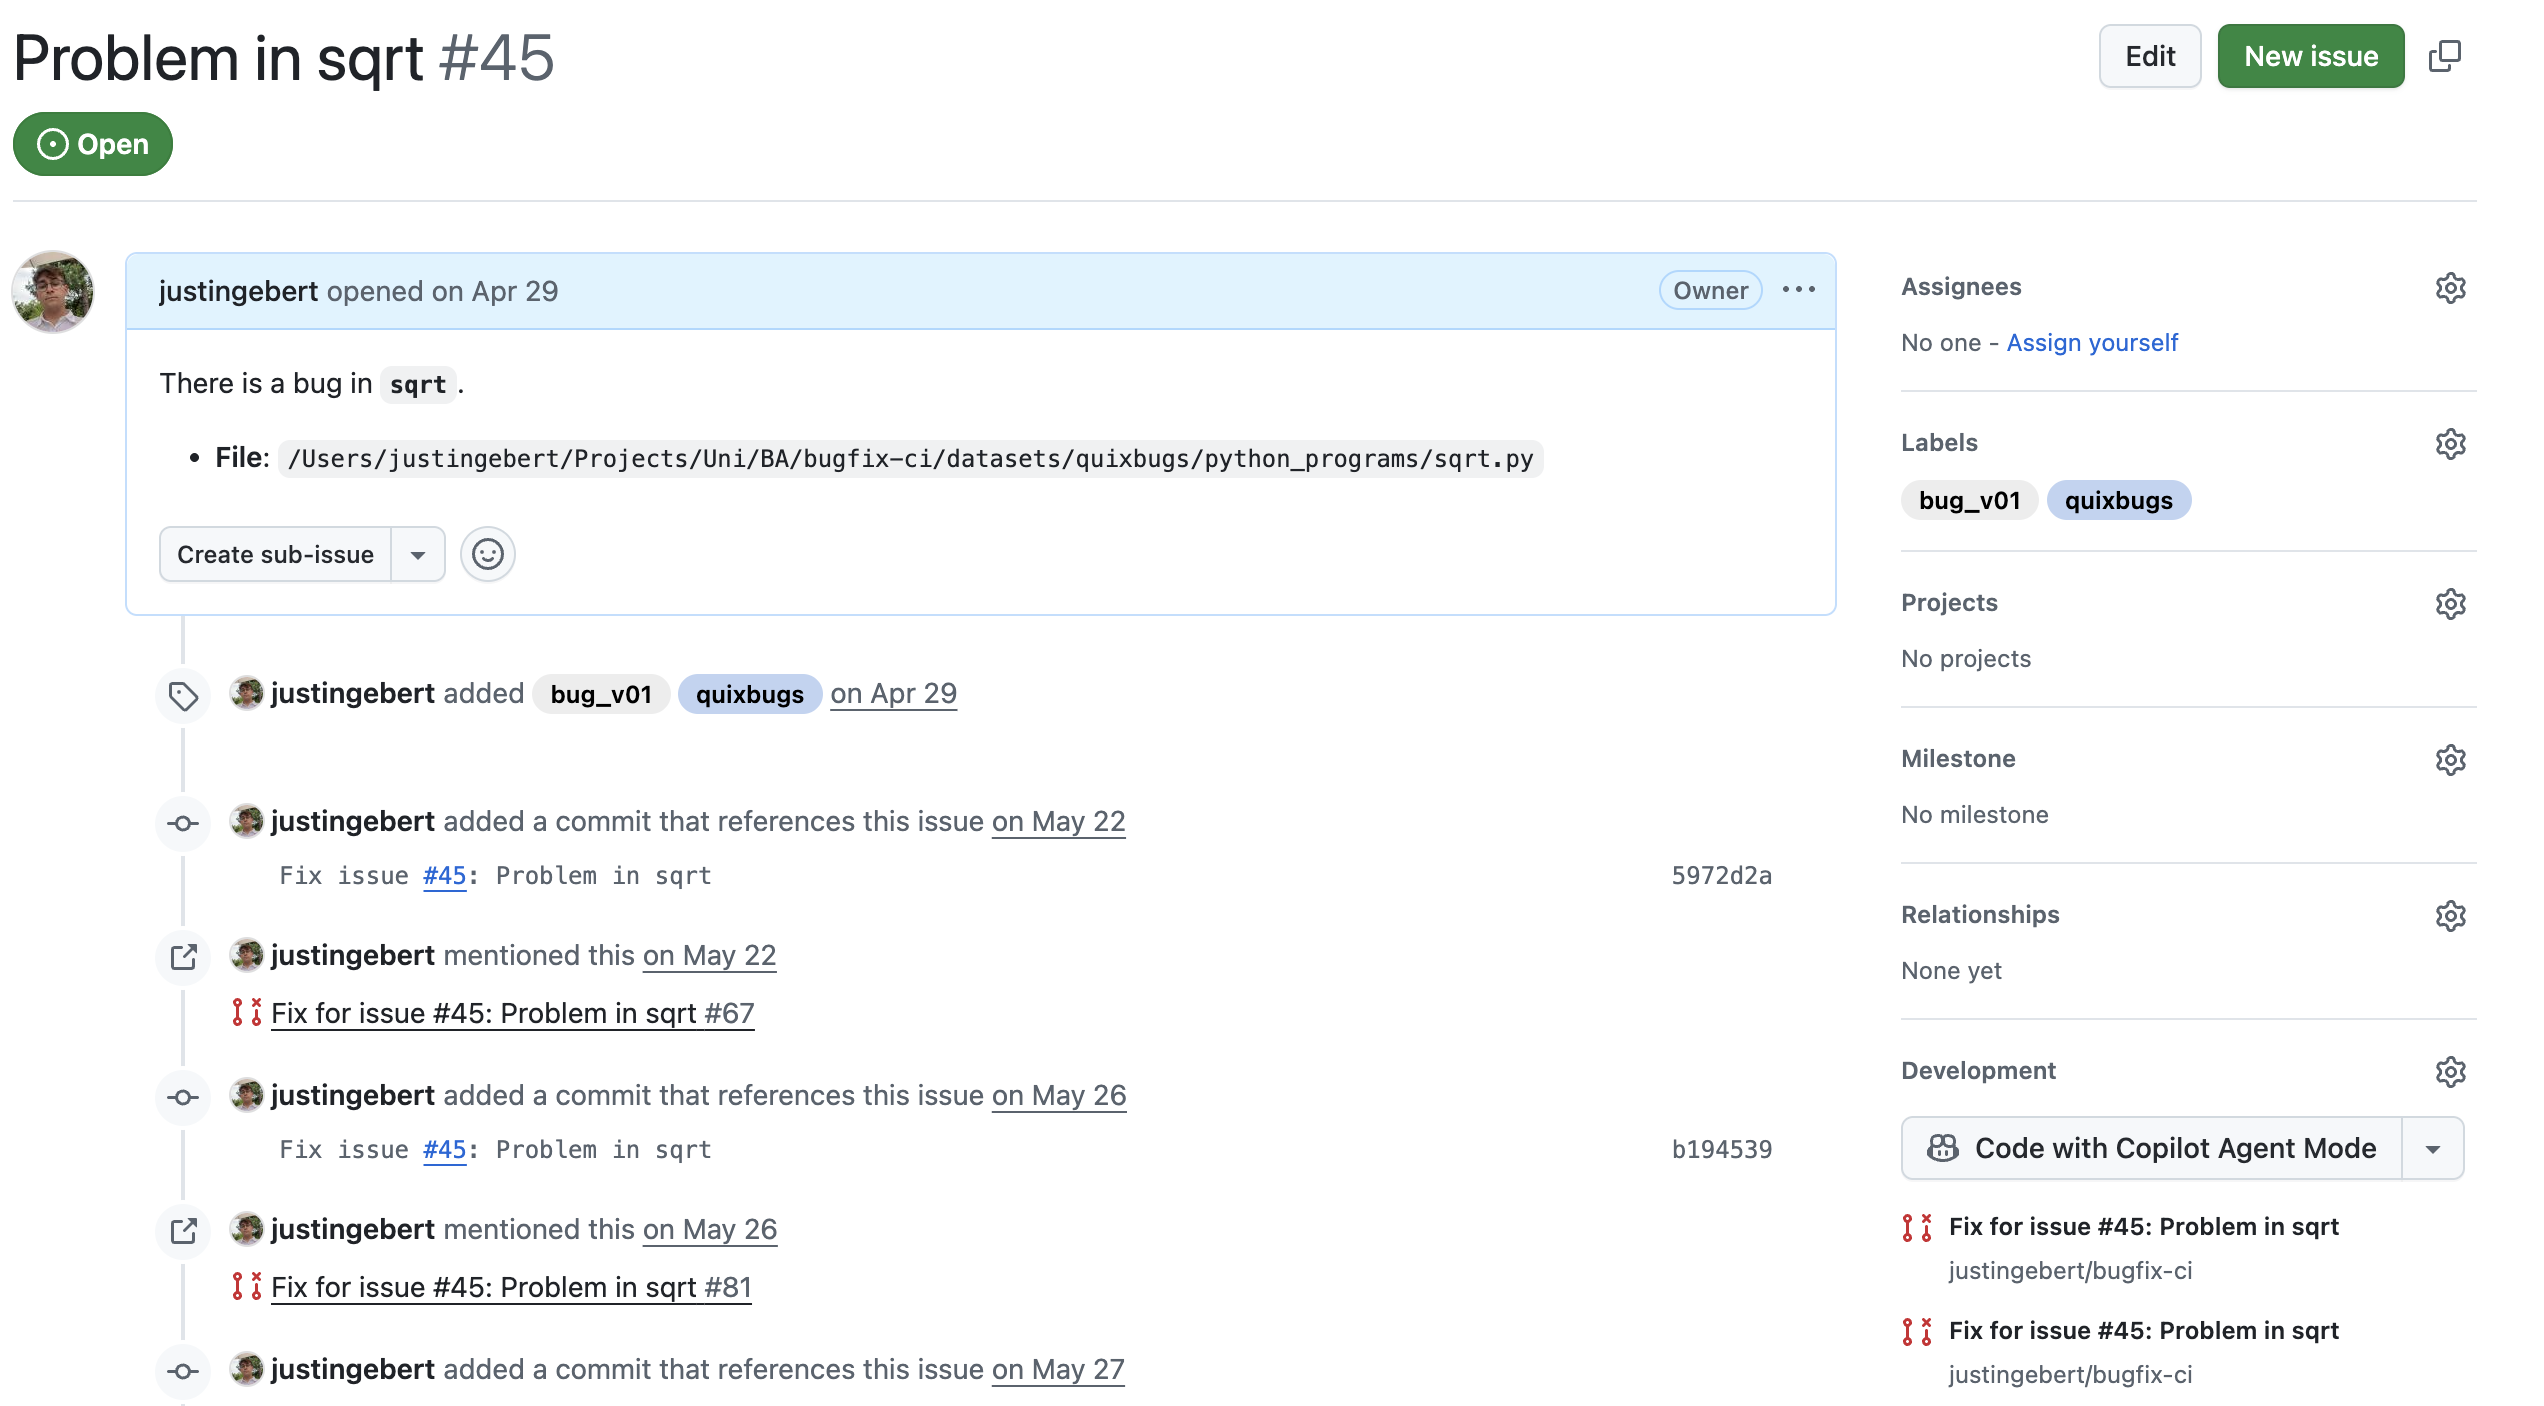
\includegraphics[width=1\textwidth]{images/github/GitHub Issue.png}
%     \caption{Example of a GitHub Issue}
%     \label{fig:gh-issue}
% \end{figure}

\section{Evaluation Results}
Our evaluation is based on the data collected during the execution of the prototype. This information is stored in the artifacts of the Github Actions run. Using the \textbf{get\_run\_data.py} script we collected the APR artifacts and the GitHub Pipeline information using the GitHub API. The script then processes the data and generates a report with the results of the evaluation. With the fetched data we calculate the metrics defined in %\ref{Evaluation}.

\begin{table}[ht]
    \centering
    \small
    \begin{tabular*}{\textwidth}{@{\extracolsep{\fill}} p{4cm} | p{2cm} | p{3cm} | p{4cm} | p{4cm} @{}}
        \toprule
        \textbf{Model} & \textbf{Repair Success Rate} & \textbf{Average Cost} & \textbf{Average Number of Attempts} & Average Execution Time \\
        \midrule
        \textbf{gemini-2.0-flash} & 0.00\% & 0.00 & 0.00 & 0.00s \\
        \bottomrule
    \end{tabular*}
    \caption{Results of evaluation}
\end{table}


with small models and attempt loop makes small models pass the whole benchmark?